\section{Symmetrische und Asymmetrische Kryptosysteme}
Es gibt 2 verschiedene Möglichkeiten für die Schlüssel von \textit{Alice} und \textit{Bob}:
\begin{enumerate}
	\item Beide besitzen den \textbf{gleichen} Schlüssel $\rightarrow$ \textbf{symmetrische Kryptosystem}
	\begin{itemize}
		\item Daher müssen beide den Schlüssel geheim halten und kennen, da sonst Eve Nachrichten entschlüsseln oder Mallory Nachrichten verschlüsseln und versenden könnte.
		\item Beide können Nachrichten \textbf{ver- und entschlüsseln}
		\item Typische Schlüssellängen sind \textbf{80-256 Bit}
		\item Die Algorithmen sind typischerweise schnell, da sie einfache Operationen (Addition, XOR, Bitshifts, Substitutionen,...) verwenden.
		\item Alle symmetrische Kryptosysteme haben das Problem des \textbf{Schlüsselaustausches}
		\item[] 
		\begin{figure}[H]
			\centering
			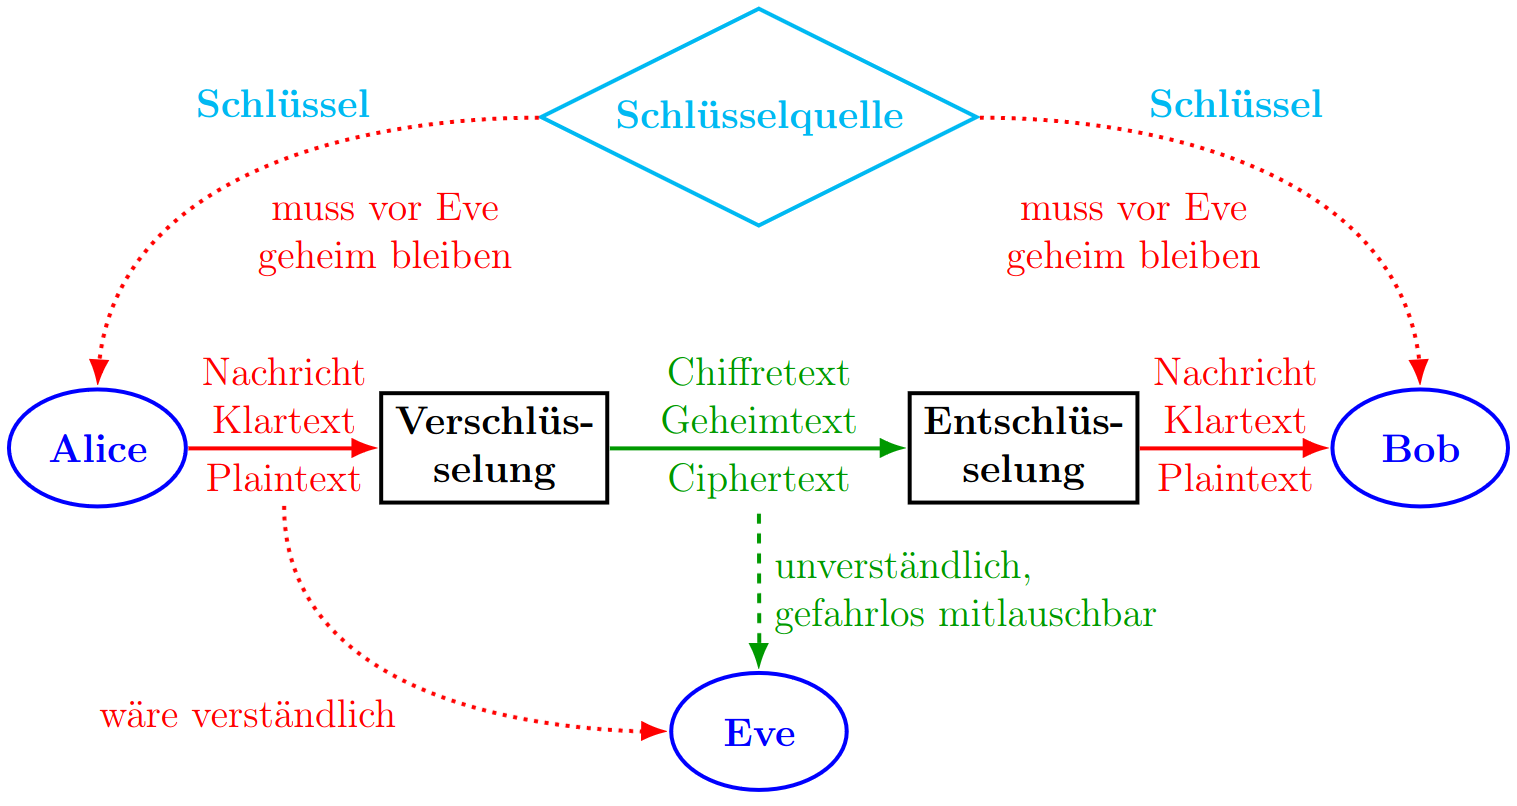
\includegraphics[width=1.0\linewidth]{figures/symmkry.png}
			\caption{Symmetrische Kryptosysteme}
		\end{figure}
	\end{itemize}
	\item Beide besitzen \textbf{verschiedene} Schlüssel $\rightarrow$ \textbf{asymmetrische Kryptosystem}
	\begin{itemize}
		\item \textit{Bob} hat einen geheimen Schlüssel, mit dem die Nachricht entschlüsselt werden kann. Der Schlüssel zum verschlüsseln ist jedem (öffentlich) bekannt. So kann Eve Nachrichteen verschlüsseln, Mallory aber nicht entschlüsseln.
		\item Alice kann ihre Nachrichten verschlüsseln, aber nicht entschlüsseln
		\item Typische Schlüssellängen sind \textbf{512-4096 Bit}
		\item Die Algorithmen sind typischerweise langsam, weil sie auf 'schwierigere' Operationen verwenden (z.B. Potenzieren).
		\item Da Alicen nur den öffentlichen Schlüssel benötigt, lösen asymmetrische Kryptosysteme das Schlüsselaustauschproblem 
		\item[] 
		\begin{figure}[H]
			\centering
			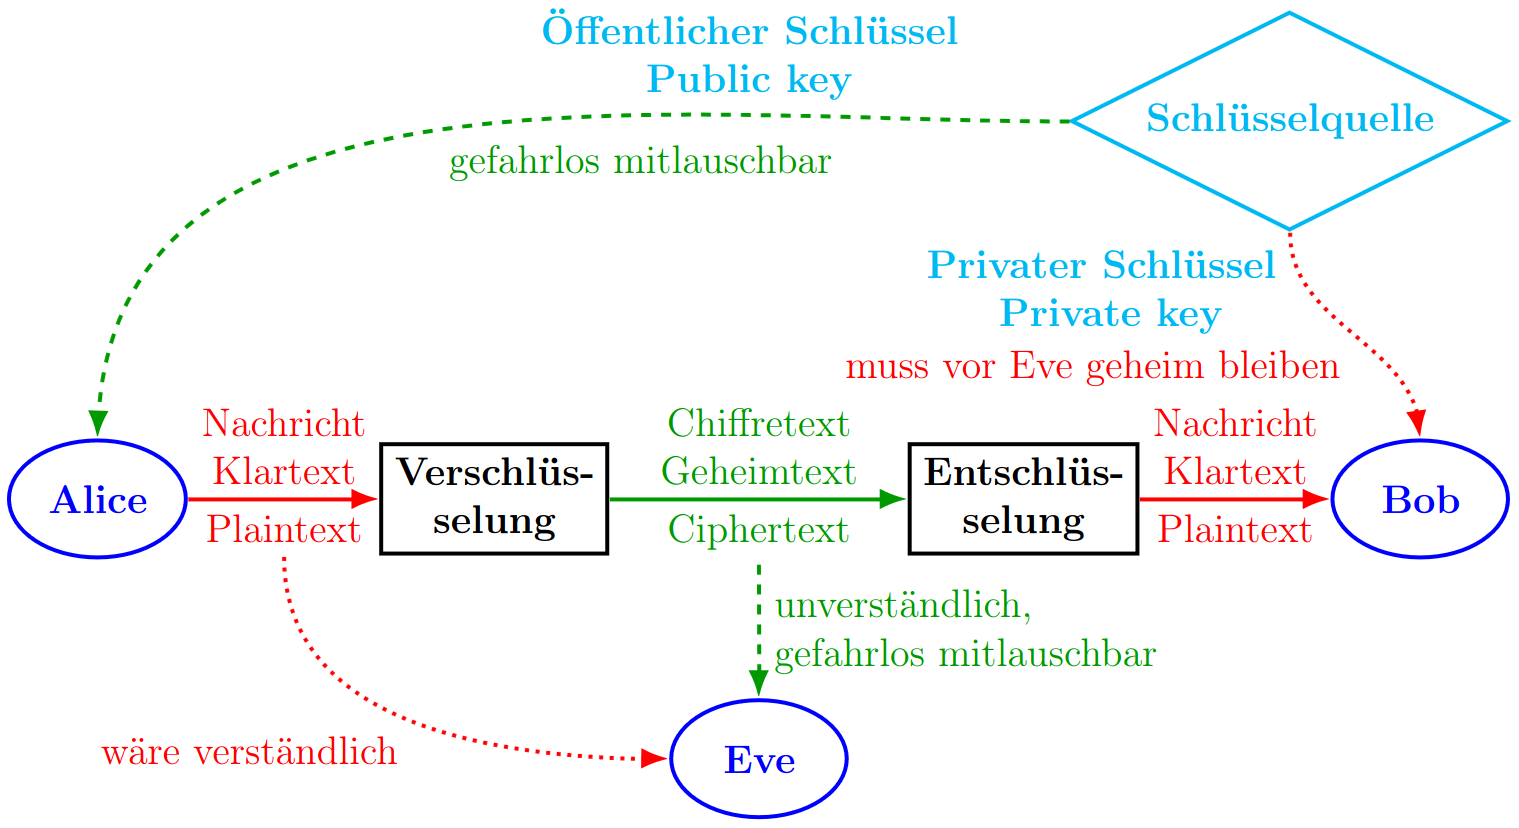
\includegraphics[width=1.0\linewidth]{figures/asymmkry.png}
			\caption{Asymmetrische Kryptosysteme}
		\end{figure}
	\end{itemize}
\end{enumerate}

Neben den bisher erwähnten Unterschieden zwischen symmetrischen und asymmetrischen Kryptosystemen gibt es noch einen weiteren Aspekt: die Anzahl der benötigten Schlüssel, um mit vielen Personen zu kommunizieren.
\begin{figure}[H]
	\centering
	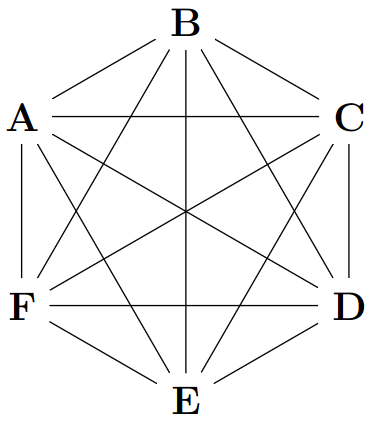
\includegraphics[width=0.2\linewidth]{figures/hexagon.png}
\end{figure}

Eine Gruppe aus 6 Personen möchte verschlüsselt kommunizieren. Dabei will jede Person in der Lage sein, mit jeder anderen Person privat zu kommunizieren.
\begin{enumerate}
	\item Anzahl der verschiedenen Schlüssel: symmetrische Kryptosysteme \\
	$\frac{6\cdot5}{2}$ = 15
	\item eine Person muss 5 Schlüssel speichern (symmetrisch)
	\item Anzahl der verschiedenen Schlüssel: asymmetrische Kryptosysteme \\
	6$\cdot$2 = 12
	\item eine Person muss 1 Schlüssel speichern (asymmetrisch)
	\item Bei n Personen
	\item[] Symmetrisch: $\dfrac{n^2}{2}$ Schlüssel insgesamt, \quad n-1 Schlüssel speichern
	\item[]  Asymmetrisch: $2 \cdot n$ Schlüssel insgesamt, \quad 1 Schlüssel speichern
\end{enumerate}








